%%%%%%%%%%%%%%%%%%%%%%%%%%%%% Define Article %%%%%%%%%%%%%%%%%%%%%%%%%%%%%%%%%%
\documentclass{article}


%%%%%%%%%%%%%%%%%%%%%%%%%%%%% Using Packages %%%%%%%%%%%%%%%%%%%%%%%%%%%%%%%%%%
\usepackage{geometry}
\usepackage{pgfplots}
\usepackage{lipsum}
\usepackage{mdframed}
\usepackage{amsthm}
\usepackage{bm}
\usepackage{titlesec}
\usepackage{tocloft}
\usepackage{ragged2e}
\usepackage{fancyhdr}
\usepackage{glossaries}
\usepackage[spanish]{babel}
\usepackage[sorting=none]{biblatex}
\usepackage[hidelinks]{hyperref}
\usepackage[all]{hypcap}
\usepackage{csquotes}
\usepackage{pdfpages}


%%%%%%%%%%%%%%%%%%%%%%%%%% Page Setting %%%%%%%%%%%%%%%%%%%%%%%%%%%%%%%%%%%%%%%
\geometry{a4paper}
\graphicspath{{img/}}
\addbibresource{bibliography.bib}
\numberwithin{figure}{section}

\fancyhf{}
\pagestyle{fancy}
\fancypagestyle{plain}{}
\lfoot{\thepage}
\fancyhead{}
\renewcommand{\headrulewidth}{0pt}

\lhead{PROYECTO FIN DE GRADO}

\titleformat{\section}
{\rmfamily\Large\raggedleft\uppercase}{\thesection.}{0.1cm}{}[{\titlerule[0.5pt]}]
\titleformat{\subsection}
    {\rmfamily\large\uppercase}{\thesubsection.}{0.1cm}{}

%%%%%%%%%%%%%%%%%%%%%%%%%%%%%%% Plotting Settings %%%%%%%%%%%%%%%%%%%%%%%%%%%%%
\usepgfplotslibrary{colorbrewer}
\pgfplotsset{width=8cm,compat=1.9}


%%%%%%%%%%%%%%%%%%%%%%%%%%%%%%% Title & Author %%%%%%%%%%%%%%%%%%%%%%%%%%%%%%%%
\title{Redes Neuronales Convolucionales}
\author{Asier Villar}


%%%%%%%%%%%%%%%%%%%%%%%%%%%%%%% Components %%%%%%%%%%%%%%%%%%%%%%%%%%%%%%%%%%%
\newcommand{\listequationsname}{\Large{Índice de ecuaciones}}
\newcommand{\myequations}[1]{
    \addcontentsline{equ}{myequations}{\protect\numberline{\theequation}#1}
}

\newcommand{\equationNote}[2]{
    \begin{align} \label{#2} \ensuremath{#1} \end{align} 
    \myequations{#2} \centering \small \textit{#2} \normalsize \justify 
}

\newlistof{myequations}{equ}{\listequationsname}
\setlength{\cftmyequationsnumwidth}{2.3em}
\setlength{\cftmyequationsindent}{1.5em}


%%%%%%%%%%%%%%%%%%%%%%%%%%%%%%% Document %%%%%%%%%%%%%%%%%%%%%%%%%%%%%%%%%%%%%
\begin{document}

    \pagenumbering{roman}
    
\includepdf[pages={1}]{frontpage.pdf}
    
\includepdf[pages={1}]{frontpage.pdf}
    \section*{Resumen}
El propósito del siguiente proyecto es investigar y desarrollar una nueva solución para el 
problema de optimización “flexible job shop scheduling problem” (FJSP), que se clasifica dentro 
de la categoría de problemas NP-hard, que son aquellos que no pueden ser resultados de forma 
exacta por un algoritmo en un tiempo de computación polinómica. El objetivo es asignar una 
serie de operaciones a un conjunto de máquinas, teniendo en cuenta una lista de restricciones 
y requisitos, como por ejemplo el tiempo de procesamiento. Por último, como resultado de lo 
anterior, se proveerá de una configuración válida, que intente minimizar el tiempo máximo de 
finalización (make span) de todas las máquinas.\medskip 

Se propone utilizar técnicas de Imitation Learning, una variante del Reinforcement learning 
que permite al modelo aprender a partir de ejemplos proporcionados por un experto. En nuestro 
caso, se estudiarán técnicas de generación de ejemplos válidos que permitan al modelo aprender 
técnicas para resolver el FJSP. La idea, es extraer configuraciones óptimas de instancias 
pequeñas generadas aleatoriamente y utilizarlas como datos de entrenamiento para un modelo, 
que pueda desarrollar una estrategia propia en base a las decisiones del experto y posteriormente 
generalizar a instancias mayores.\medskip 

El objetivo es mejorar la velocidad en la que se ofrecen planificaciones cercanas al óptimo, 
ya que con este planteamiento no será necesario explorar todo el espacio de soluciones. Otro 
de los beneficios es la adaptabilidad a variaciones del problema dinámicamente, como cambios 
en los tiempos de procesamiento o la incorporación de nuevas operaciones. Teniendo esto en 
cuenta, se espera obtener una solución en tiempo lineal que no se desvíe excesivamente del 
óptimo y que pueda aplicarse a diferentes escenarios industriales e incluso en consonancia 
con otras técnicas.

\section*{Descriptores}
Reinforcement Learning, Imitation Learning, FJSP, Redes Neuronales, MLOPS
\pagebreak 
    \tableofcontents
\listoftables
\listoffigures
\pagebreak 
 

    \pagenumbering{arabic}
    \section{Introducción}
La planificación de la producción es una disciplina clave en la gestión de 
activos y se utiliza para determinar la forma más eficiente de asignar 
recursos, como maquinaria, mano de obra y tiempo, con el fin de alcanzar 
los objetivos de producción. Es un proceso que implica la toma de decisiones 
sobre qué recursos, cuánto, cuándo y cómo producirlos, con el objetivo de optimizar la 
utilización de los elementos disponibles, maximizando la eficiencia y rentabilidad 
del proceso de producción. La planificación de la producción se aplica en una 
amplia gama de sectores y áreas de negocio, incluyendo la fabricación, la logística, 
el transporte, la distribución y la gestión de la cadena de suministro, entre otros.\medskip

La importancia de la planificación de la producción radica en su capacidad para mejorar 
la eficiencia mediante una buena gestión de las operaciones, lo que puede tener un impacto 
significativo en la rentabilidad y competitividad de las empresas. Una planificación de 
producción efectiva debe optimizar la asignación de recursos, minimizar los tiempos de 
inactividad, reducir los costos de producción y maximizar el cumplimiento de los plazos 
de entrega en la medida de lo posible. Esto lo que resulta es en una mayor eficiencia operativa 
y una mejor calidad del producto o servicio.\medskip

Sin embargo, la planificación de la producción es un problema complejo debido a la gran 
cantidad de variables y restricciones que deben tenerse en cuenta, como los tiempos de 
procesamiento, las capacidades de los recursos, las restricciones de almacenamiento y 
transporte y las demandas de los clientes, entre otros. Tradicionalmente, este problema 
se ha abordado utilizando enfoques heurísticos y algoritmos de optimización, como el 
Job Shop Scheduling Problem (JSP) y el Flexible Shop Scheduling Problem (FJSP), que son problemas 
combinatorios y conocidos por ser NP-Hard, lo que implica que no existen algoritmos eficientes 
para encontrar soluciones óptimas en un tiempo razonable.\medskip

Un problema NP-Hard es un tipo de problema de optimización en el cual no se conocen algoritmos 
eficientes que puedan encontrar una solución óptima en un tiempo polinómico. Esto implica que a 
medida que el tamaño del problema aumenta, el tiempo de cómputo necesario para encontrar una 
solución óptima también se vuelve prohibitivamente alto. Estos problemas son considerados de 
gran complejidad y representan un desafío significativo para la investigación en ciencias de 
la computación. La importancia de identificar un problema como NP-Hard radica en que a menudo 
tecnicas utilizadas para un problema pueden ser aplicados a otros problemas NP-Hard. Esto se debe a que 
muchos problemas NP-Hard comparten estructuras y patrones similares, lo que permite la 
transferencia de conocimientos y técnicas de un problema a otro. Por lo tanto, encontrar 
soluciones eficientes o aproximadas para un problema NP-Hard particular puede tener un impacto 
significativo en la resolución de otros problemas que enfrentan desafíos similares\medskip

En los últimos años, ha surgido el Imitation Learning como una prometedora técnica de aprendizaje 
automático. El Imitation Learning se basa en el concepto de aprender de la experiencia de expertos 
humanos o de sistemas de planificación previamente establecidos, y luego utilizar ese conocimiento para 
guiar la toma de decisiones en situaciones similares. Esto se puede lograr a través de enfoques 
supervisados, donde se entrena a un modelo para imitar las acciones de expertos humanos, o 
a través de enfoques de Reinforcement Learning (RL), donde se permite que un modelo aprenda a 
partir de la retroalimentación y la interacción con el entorno.\medskip

En este contexto, el presente trabajo se enfoca en el desarrollo de un sistema de planificación 
de la producción basado en Imitation Learning, utilizando técnicas de aprendizaje supervisado y RL. 
Se busca explorar cómo estas técnicas pueden aplicarse a la planificación de la producción, teniendo 
en cuenta los desafíos y la complejidad de este problema. A través del estudio y análisis de 
diferentes enfoques y metodologías, se pretende contribuir al campo de la planificación de la 
producción utilizando técnicas de inteligencia artificial y aprendizaje automático, con el objetivo 
de mejorar la eficiencia y la toma de decisiones en procesos industriales.\medskip

\subsection{Motivación}
La planificación de la producción es un desafío constante en la industria, ya que puede tener 
un impacto significativo en la eficiencia, la productividad y la rentabilidad de las operaciones 
de fabricación. Sin embargo, muchos de los problemas de planificación de la producción en la 
industria, como el Job Shop Scheduling Problem (JSP) y el Flexible Job Shop Scheduling Problem (FJSP), 
son conocidos por su alta complejidad y la falta de soluciones eficientes. Esto puede resultar 
en cuellos de botella, retrasos en la producción y costos innecesarios.\medskip

Es crucial encontrar soluciones innovadoras y eficientes que puedan abordar 
los desafíos complejos asociados con la planificación de la producción en entornos que enfrentan 
problemas NP-Hard. Además, la aplicación de enfoques de inteligencia artificial y aprendizaje 
automático en la planificación de la producción ha ganado cada vez más atención en la industria 
debido a su potencial para encontrar soluciones aproximadas en tiempo real y adaptarse a 
entornos dinámicos.\medskip

La motivación de este proyecto radica en la necesidad de desarrollar enfoques de Imitation 
Learning, una rama del aprendizaje automático que se basa en la imitación de comportamientos 
de expertos, para abordar los desafíos de la planificación de la producción en la industria. 
Estos enfoques tienen el potencial de mejorar la eficiencia y la productividad de las operaciones 
de fabricación al encontrar soluciones eficientes y adaptativas en tiempo real. Además, las 
soluciones desarrolladas en el contexto del JSP y el FJSP podrían tener aplicaciones amplias 
en otros problemas NP-Hard que enfrenta la industria, como la logística, la programación de 
tareas o la asignación de recursos, lo que podría tener un impacto significativo en la 
optimización de procesos y la competitividad de las empresas en la industria.

\subsection{Explicación del problema}
El Flexible job shop scheduling problem (FJSP), es un desafío de optimización combinatoria 
que se encuentra en el campo de la la gestión de la producción. En este problema, se busca determinar 
la secuencia óptima de operaciones a realizar en una serie de máquinas, con el objetivo de minimizar el 
tiempo total de producción o maximizar la eficiencia del sistema. A diferencia del Job shop scheduling 
problem (JSP), en el que cada operación tiene una ruta de procesamiento fija, las operaciones pueden ser 
procesadas en varias máquinas diferentes. Además, adicionalmente las operaciones estan agrupadas 
dentro de un trabajo, que es un conjunto de operaciones que deben ser procesadas en una secuencia
específica.\medskip

Existen dos restricción temporales que especifican cuándo puede comenzar 
cada operación: una operación no puede comenzar hasta que se hayan completado todas las operaciones
anteriores de la misma tarea y no puede comenzar hasta que se hayan completado todas las operaciones
anteriores de la misma máquina. El objetivo del problema es asignar las operaciones a las máquinas y determinar el orden de procesamiento 
del sistema manera óptima, teniendo en cuenta las restricciones temporales y los recursos disponibles, 
de manera que se minimice el tiempo total de producción. El tiempo total de producción se refiere al
tiempo de finalización de la máquina más lenta, que se calcula sumando el tiempo de procesamiento 
de todas las operaciones y el gap que estas generan.\medskip

Para ilustrar el problema, supongamos que tenemos una fabrica que produce tres tipos de productos
que se definen como los trabajos: A, B y C. Contamos con tres máquinas: M1, M2, M3 y M4 
y cada producto requiere hacer ciertas operaciones de procesamiento en estas máquinas en 
un orden específico. Las operaciones y los tiempos de procesamiento estimados para cada 
producto en cada máquina son los siguientes: 

\begin{table}[ht]
    \caption{Tiempos de procesamiento estimados para cada producto} 
    \centering 
    \begin{tabular}{ccccccccc}  

    \toprule
    \multirow{2}{*}{\parbox[c]{.2\linewidth}{\centering Maquina ID}} & 
    \multicolumn{2}{c}{Trabajo A} && 
    \multicolumn{2}{c}{Trabajo B} && 
    \multicolumn{2}{c}{Trabajo C} \\ 

    \cmidrule{2-3} \cmidrule{5-6} \cmidrule{8-9}
     & {\centering OP 1} & {OP 2} && {OP 3} & {OP 4} && {OP 5}\\

    \midrule
    Máquina 1 & 4 UT & --   && 3 UT & 7 UT && 1 UT & -- \\
    Máquina 2 & 3 UT & 2 UT && 2 UT & 2 UT && 6 UT & -- \\
    Máquina 3 & 2 UT & 1 UT && --   & 5 UT && 2 UT & -- \\  
    Máquina 4 & --   & 3 UT && 4 UT & 8 UT && 4 UT & -- \\ 
    \bottomrule
    
    \end{tabular}
\end{table}

\medskip

Aquí, cada operación se identifica con un número y el tipo de procesamiento se mide en Unidades temporales
(UD). Las operaciones que no se pueden realizar en una máquina se identifican con un guión (-), lo que 
significa que en este ejemplo la máquina 1 podría procesar las operaciones 1, 3, 4 y 5 pero 
no la operación 2. Una vez entendida la distribución de tiempos de procesamiento, podemos visualizar
el resultado de la planificación en el siguiente diagrama, donde cada caja representa una operación 
y cada línea representa una máquina.

\begin{figure}[ht]
    \centering
    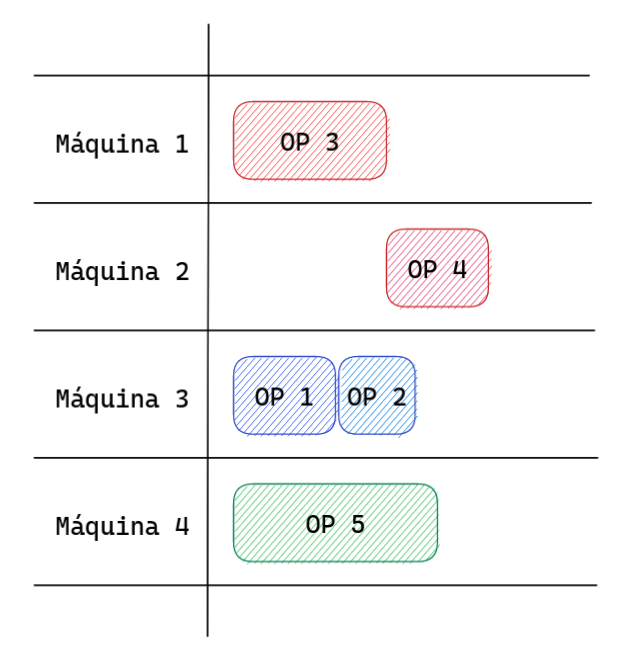
\includegraphics[scale=0.40]{ejemplo.png}
    \caption{Ejemplo de planificación óptima}
    \label{fig:example-solution}
\end{figure}

La distribución final de tiempos para cada máquina es la siguiente: 
\begin{itemize}
    \item \textbf{maquina 1}, OP 3 (3 UT) + 0 GAP = 3 UT 
    \item \textbf{maquina 2}, OP 4 (2 UT) + 3 GAP = 5 UT 
    \item \textbf{maquina 3}, OP 1 (2 UT) + OP 2 (1 UT) + 0 GAP = 3 UT 
    \item \textbf{maquina 4}, OP 5 (4 UT) + 0 GAP = 4 UT. 
\end{itemize}

Ya que el tiempo total de producción es el tiempo de finalización de la máquina más lenta, 
que es la máquina 2, son 5 UT. Notese que el gap de la máquina 2 es deribado de la dependencia
existente entre la operación 4 y la operación 3 por petenercer ambos al trabajo B, 
por lo tanto, antes de que dicha maquina empiece con la operacion 4 tiene que esperar 
a que se procese la máquina 1.

\subsection{Estructura de la memoria}



\pagebreak
    \section{Antecedentes y justificación}
El objetivo de esta seccion es describir las condiciones del entorno en el que se lleva a cabo 
el proyecto, se recopilarán datos e información sobre la situación actual en lo que respecta al FJSP, 
incluyendo la utilización de diferentes tecnicas que han sido utilizadas historicamente para su resolución. 
Para ello, se revisará el estado del arte y las últimas tendencias en este campo, con el fin de obtener una 
mejor comprensión del problema y explicar la oportunidad de realizar nuevos aportes en esta área de investigación.


\subsection{Estado del arte}
\subsubsection{Metodos exactos}
Los métodos exactos se basan en la resolución matemática del problema, y pueden garantizar la 
obtención de soluciones óptimas en teoría. Sin embargo, estos métodos suelen ser computacionalmente 
costosos y, por lo tanto, se aplican principalmente a problemas de tamaño reducido.\medskip

En el caso del FJSP, algunos métodos exactos que se han utilizado incluyen la programación 
lineal de enteros mixta (MILP)\cite{milp}, que modela el problema como un conjunto de restricciones lineales y 
una función objetivo lineal, y la programación por restricciones (CP)\cite{wikiCP}, que reduce el problema a
un conjunto de restricciones lógicas y utiliza técnicas de búsqueda para encontrar soluciones que satisfagan 
todas las restricciones. Existen aplicaciones hechas por google como Ortools\cite{ortools}
o por IBM como CPLEX\cite{cplex}, que son ejemplos de soluciones que utilizan estos métodos exactos para resolver
problemas de optimización. Estas aplicaciones son muy útiles para resolver instancias de tamaño reducido,
pero no son capaces de resolver instancias de tamaño grande, debido a la gigantesca dimensionalidad que
implica el resolver este tipo de problemas por métodos exactos.


\subsubsection{Metodos heurísticos}
Un método heurístico es un algoritmo o técnica de búsqueda que está diseñado para encontrar 
soluciones aproximadas a problemas de optimización, cuando las soluciones exactas son difíciles 
de encontrar. Los métodos heurísticos son útiles cuando el tiempo y los recursos son limitados, 
y cuando el problema a resolver es demasiado complejo para ser resuelto por medios exactos. 
Estos métodos se basan en la experiencia y el conocimiento previo para generar soluciones que 
son buenas pero no necesariamente óptimas. Los métodos heurísticos pueden ser aplicados a una 
amplia variedad de problemas de optimización, incluyendo el FJSP.\medskip

En el caso del FJSP, existen diferentes métodos heurísticos que se han utilizado con éxito 
para encontrar soluciones aproximadas. Un ejemplo es el algoritmo de búsqueda tabú, 
que se basa en la exploración de soluciones vecinas para encontrar soluciones cada vez mejores. 
Otro ejemplo es el algoritmo de búsqueda local, que busca soluciones iterativamente en una 
vecindad de soluciones. También se ha utilizado el enfoque basado en la construcción de 
soluciones parciales, donde se construyen soluciones en etapas, utilizando información previa 
y reglas heurísticas para guiar el proceso de construcción. Todos estos métodos heurísticos 
han demostrado ser efectivos para resolver el problema de FJSP, y se pueden adaptar y mejorar 
para abordar variantes más complejas del problema.

\subsubsection{Algoritmos genéticos}
Los algoritmos genéticos son una técnica de optimización inspirada en la evolución biológica.
Estos algoritmos imitan el proceso de selección natural, reproducción y mutación en la búsqueda 
de soluciones óptimas o cercanas a la óptima para problemas de optimización combinatoria. La 
idea básica de los algoritmos genéticos es utilizar la selección natural para encontrar soluciones
mejores a través de la generación de nuevas soluciones a partir de soluciones existentes y la 
aplicación de operadores de cruce y mutación.\medskip

En la literatura, estos algoritmos han sido ampliamente utilizados y han demostrado ser 
efectivos para encontrar soluciones de alta calidad. La representación cromosómica utilizada 
en los algoritmos genéticos se basa en la codificación de una solución del problema de FJSP 
como una cadena de genes, y los operadores genéticos como el cruzo o la mutación, se aplican 
para producir nuevas soluciones o realizar ligeros cambios en aquellas ya existentes. Una de 
sus principales ventajas es que pueden manejar fácilmente múltiples objetivos y restricciones 
adicionales, y son capaces de explorar ampliamente el espacio de soluciones.\medskip

En cambio uno de sus problemas es que los algoritmos genéticos pueden requerir una gran cantidad 
de tiempo y esfuerzo para encontrar soluciones aceptables, y no siempre garantizan encontrar la 
mejor solución posible. Además, pueden requerir ajustes cuidadosos de los parámetros y una 
cuidadosa selección de operadores para funcionar bien en diferentes instancias del problema y 
tienen tendencia a sufrir de prematura convergencia lo que genera dificultades para escapar de 
óptimos locales.

\subsubsection{Algoritmos híbridos}
Los algoritmos híbridos son aquellos que combinan dos o más algoritmos que resuelven el mismo problema. 
En el caso del FJSP, los algoritmos híbridos combinan diferentes técnicas de optimización para encontrar 
soluciones. Por ejemplo, un algoritmo híbrido podría combinar un algoritmo genético con un algoritmo de 
búsqueda local para aprovechar las ventajas de ambos y mejorar la calidad de las soluciones encontradas.

\subsubsection{Redes neuronales}
Las redes neuronales son una clase de algoritmos de aprendizaje automático inspirados en la 
estructura y el funcionamiento del cerebro humano. Estas redes están formadas por múltiples 
capas de neuronas interconectadas que procesan información para resolver problemas de clasificación, 
regresión, reconocimiento de patrones, entre otros.\medskip

En el contexto del FJSP, las redes neuronales pueden ser utilizadas para aprender patrones en los datos
de entrada del problema, como la secuencia de tareas y las restricciones de precedencia. Esto puede 
ayudar a generar soluciones de alta calidad al FJSP, incluso para instancias de problemas grandes y 
complejas. Además, las redes neuronales también pueden ser entrenadas para mejorar la calidad de las 
soluciones generadas por otros algoritmos de optimización, como los algoritmos genéticos y los métodos 
heurísticos.\medskip

La principal ventaja de las redes neuronales es su capacidad para manejar datos no lineales y ruidosos, 
y para detectar patrones complejos en los datos de entrada. Sin embargo, las redes neuronales también 
pueden presentar desafíos en el entrenamiento y ajuste de los hiperparámetros, y pueden ser propensas 
a sobreajuste si no se controlan adecuadamente, pero incluso con esos inconvenientes son una de las 
técnicas más prometedoras para el FJSP y pueden ser utilizadas en combinación con otras técnicas de 
optimización para mejorar la calidad de las soluciones.

\subsubsection{Reinforcement learning}
El aprendizaje por refuerzo es una técnica de aprendizaje que se basa en la idea de que un agente 
interactúa con un entorno para aprender a tomar decisiones óptimas en función de las recompensa 
recibida por sus acciones. En el aprendizaje por refuerzo, el agente aprende a través de la 
experiencia, probando diferentes acciones y observando las recompensas asociadas con cada una 
de ellas, con el objetivo de maximizar la recompensa total a largo plazo.\medskip

En el contexto del FJSP, el aprendizaje por refuerzo puede ser utilizado para entrenar a un 
agente que toma decisiones secuenciales sobre la asignación de tareas a máquinas y la 
planificación de la secuencia de tareas, con el objetivo de minimizar el tiempo total de producción. 
Una de las principales ventajas del aprendizaje por refuerzo es su capacidad para aprender directamente 
de la experiencia, sin la necesidad de un modelo matemático explícito del problema, lo que lo hace 
útil para resolver problemas complejos y mal definidos como el FJSP. Sin embargo, el aprendizaje 
por refuerzo también presenta desafíos en la definición de la función de recompensa y en la 
selección de la política óptima que maximiza la misma. Además, requiere de una gran cantidad de tiempo 
y recursos computacionales para entrenar al agente en instancias del problema de FJSP grandes y complejas.

\subsubsection{Imitation learning}
El aprendizaje por imitación es una técnica de aprendizaje por refuerzo en la que un modelo aprende
a partir de ejemplos proporcionados por un experto. En el aprendizaje por imitación, el modelo trata
de imitar la forma en que el experto realiza una determinada tarea, utilizando los ejemplos como guía.
Además, el experto no tiene por qué ser una persona física, también es posible utilizar algoritmos de
optimización para generar soluciones de alta calidad, y luego utilizar estas soluciones como ejemplos
de entrenamiento para el aprendizaje por imitación.\medskip

Esta técnica puede ser utilizada para aprender a generar soluciones de alta calidad a partir de 
configuraciones previamente resueltas por un experto, esto es gracias a que el modelo es capaz de 
identificar patrones y características comunes en las soluciones óptimas del problema. Luego, el 
modelo puede ser utilizado para generar nuevas soluciones que imiten el comportamiento del experto 
humano. Una de las principales ventajas del aprendizaje por imitación es que los datos que se le 
ofrece son soluciones de alta calidad, lo que agiliza el entrenamiento sin requerir la optimización 
iterativa del problema. 

\subsubsection{Ensenble learning}
Un ensamblador en machine learning, también conocido como ensemble learning, es una técnica que 
combina múltiples modelos de aprendizaje automático para mejorar la precisión y estabilidad de 
las predicciones. Cada uno de estos algoritmos puede tener fortalezas y debilidades en términos 
de su capacidad para encontrar soluciones óptimas en diferentes instancias del problema. Al 
combinarlos en un ensamblador, se pueden aprovechar las fortalezas de cada uno de ellos y obtener
soluciones más robustas y de mejor calidad.\medskip

Cada modelo produce una predicción diferente y las predicciones de los distintos modelos se combinan 
para obtener una única predicción. Existen diferentes tipos de ensemblers como 
el ensamble por votación, el ensamble por bagging, el ensamble por boosting y el ensamble por stacking.
Cada uno de estos ensemblers representa una estrategia diferente para combinar las predicciones de
los distintos modelos, por ejemplo en el ensamble por votación, cada modelo vota por la accion a la que predice, 
y la resultante con mayor número de votos es la predicción final.

\subsection{Antecedentes}
Una vez terminada la investigación sobre el estado actual del problema, se explorarán diversas ideas 
y reflexiones que han supuesto un impacto previo para la motivación de este trabajo. A nivel de industria, se 
presentan dos principales desafíos que enfrenta este problema de optimización combinatoria: la utilidad de los 
algoritmos metaheurísticos en escenarios online, y la capacidad de los usuarios para expresar claramente las 
funcionalidades y restricciones del problema. En ambos casos, se explicaran los antecedentes que han motivado
el desarrollo de este trabajo y se presentarán las principales ideas que se han explorado en la literatura.\medskip

De acuerdo a la investigacion realizada con anterioridad, si bien los metaheurísticos son ampliamente utilizados 
en la solución de problemas de optimización, su velocidad y practicidad en situaciones reales pueden ser limitadas, 
ya que a menudo requieren de una gran cantidad de iteraciones y evaluaciones para encontrar una solución óptima. 
Esto puede resultar en un tiempo de ejecución prolongado, lo que no es adecuado para aplicaciones en tiempo real 
o decisiones a corto plazo. El buscar un sistema que pueda resolver el problema en tiempo real es un desafío 
importante para la industria, ya que la capacidad de tomar decisiones rápidas y eficientes es crucial.\medskip 

Otro de los desafíos que enfrenta la industria es la capacidad de los usuarios para expresar claramente las
funcionalidades y restricciones del problema. En la mayoría de las situaciones, los usuarios no tienen conocimientos
suficientes o la capacidad de expresar las restricciones del problema de forma precisa, pero si son capaces de
indentificar las soluciones óptimas. Por ejemplo, en el caso de la logística en el transporte, donde una empresa 
de transporte de mercancías puede tener una idea clara de cómo quisiera asignar los vehículos a las rutas de 
entrega para minimizar los tiempos de viaje y los costos de combustible. Sin embargo, expresar todas las 
restricciones y consideraciones relacionadas con la capacidad de los vehículos, los horarios de los conductores, 
las restricciones de tiempo y las regulaciones de tráfico en una formulación matemática puede resultar complicado 
y requerir un conocimiento técnico multidisciplinario.\medskip

En este escenario, los operadores con experiencia podrían proporcionar soluciones de alta calidad, que luego 
podrían ser utilizados como datos de entrenamiento para un modelo de Imitation learning. El modelo aprendería 
a imitar el comportamiento del experto a partir de estos ejemplos, capturando así la intuición y el conocimiento 
tácito que tienen los usuarios, pero que pueden tener dificultades para expresar de manera formal. De esta manera, 
se podra abordar la brecha entre el conocimiento tácito de los operadores y la representación formal de las 
funcionalidades y restricciones del problema, permitiendo desarrollar soluciones más precisas y efectivas.\medskip

En conclusión, la idea de aprovechar el conocimiento tácito de los expertos en la resolución de problemas de 
optimización combinatoria a través de técnicas de inteligencia artificial ofrece un prometedor potencial. La 
capacidad de capturar el conocimiento de los usuarios que enfrentan dificultades en la formulación
del problema, puede ser clave para mejorar la efectividad en la toma de decisiones para procesos complejos. Además,
si gracias a estas técnicas logramos inferir una estrategia para construir soluciones a partir de ese conocimiento,
podríamos solucionar colateralmente el problema del tiempo de ejecución que habíamos identificado en los algoritmos 
metaheurísticos, ya que no necesitaríamos explorar todo el espacio de soluiciones para encontrar una solución óptima,
lo que nos permitiría reducir el tiempo de ejecución de los algoritmos drasticamente.



\pagebreak
    \section{Objetivos y alcance}
En esta sección se introducen los objetivos en los que va consistir el
proyecto, habiéndose realizado una division entre el principal y los
secundarios. Ademas de ello, se presentan los elementos que forman el alcance,
asi como se comentaran otros que no forman parte de este.

\subsection{Objetivos generales}
El objetivo del proyecto es desarrollar un nuevo método para resolver el FJSP a
partir de ejemplos de soluciones proporcionadas por un experto. El método se
basará en el uso de modelos de Deep Learning, los cuales serán entrenados para
imitar el comportamiento de un experto y desarrollar una estrategia propia.
Esto le permitirá tomar decisiones sobre instancias nunca antes vistas en un
tiempo de ejecución reducido. Para ello, a continuación se describen los
objetivos específicos:

\begin{itemize}
    \item \textbf{Identificar al experto:} el primer objetivo consta de seleccionar un
          experto capaz de generar una muestra representativa de las configuraciones y decisiones
          optimas a realizar en diferentes situaciones. Estos ejemplos servirán como datos
          de entrenamiento para el modelo de Deep learning.
    \item \textbf{Modelar el problema:} buscar una representación adecuada que permita gestionar
          las configuraciones y decisiones tomadas por el experto. Al tratarse de un modelo basado en
          Imitation Learning, es necesario definir un environment que permita la interacción entre el
          modelo y el estado del problema.
    \item \textbf{Entrenar el modelo:} utilizando los ejemplos recopilados, se debe entrenar
          el modelo de Deep learning para que pueda aprender a imitar el comportamiento
          del experto en la toma de decisiones. Esto implica ajustar los parámetros del modelo para
          minimizar el error entre las salidas predichas por el modelo y las decisiones tomadas por
          el experto en los ejemplos de entrenamiento.
    \item \textbf{Evaluar el modelo:} comprobar que el modelo ha inferido correctamente
          los patrones de comportamiento del experto, se debe evaluar su rendimiento en situaciones
          nuevas. Para ello, se utilizarán instancias de prueba que no han sido utilizadas en el
          entrenamiento del modelo. Además, se estudiarán diferentes métricas que permitan evaluar
          correctamente el desempeño del modelo. Por último, se tendrán en cuenta aspectos adicionales
          como el tiempo de ejecución del modelo.
    \item \textbf{Optimizar el modelo:} cuando el desempeño del modelo no es satisfactorio o
          se intuyen posibles mejoras, se deben identificar que áreas el modelo muestra dificultades y realizar ajustes
          en su arquitectura, parámetros o datos de entrenamiento para mejorar su rendimiento. Esto
          se puede lograr mediante el aumento del volumen del entrenamiento, monitorizando el desempeño
          del mismo o mediante la optimización de los hiperparámetros de entrenamiento.
    \item \textbf{Desplegar el modelo:} por último, se debe implementar el modelo dentro de
          una aplicación que permita su uso por parte de los usuarios. Esta aplicación debe ser capaz
          de cargar diferentes configuraciones del problema, ejecutar el modelo y graficar los resultados
          obtenidos.
\end{itemize}

\subsection{Alcance}
En esta sección se definen los límites del proyecto, estableciendo lo que está
incluido y excluido dentro mismo. Se describirá de manera detallada las
actividades que forman parte del desarrollo final, así como aquellos elementos
que no están incluidos en el alcance del proyecto. Esta sección es fundamental
para tener una comprensión clara y evitar posibles malentendidos o confusiones
durante su ejecución.

\subsubsection{Dentro del alcance}
\begin{itemize}
    \item \textbf{Variante del problema:} la versión del problema que se abordará en este proyecto
          es una variante del JSP. Este problema se caracteriza por una mayor
          complejidad debido a que una misma tarea puede ser ejecutada por diferentes máquinas.
    \item \textbf{Generación de ejemplos de entrenamiento:} el set de entrenamiento estará compuesto
          por instancias generadas de forma aleatoria, estas instancias serán generadas sintéticamente
          utilizando un algoritmo que crea instancias de problemas FJSP con tiempos de preparación.
    \item \textbf{Análisis de resultados mediante benchmarks:} se utilizarán benchmarks
          específicos para medir el rendimiento del modelo. Estos benchmarks son conjuntos de instancias
          especialmente difíciles, que reflejan de manera objetiva el desempeño del modelo.
    \item \textbf{Comparación contra técnicas actuales:} durante las diferentes fases del desarrollo,
          se monitorizara el rendimiento del método para compararlo posteriormente con las técnicas actuales
          que se emplean en el estado del arte para la resolución del problema.
    \item \textbf{Desarrollo de una aplicación web sencilla:} la aplicación final contará con una interfaz
          web que permita visualizar los resultados obtenidos por el modelo. Esta aplicación
          permitirá cargar diferentes configuraciones del problema, ejecutar el modelo y visualizar
          un Gantt con las tareas asignadas a cada máquina.
\end{itemize}

\subsubsection{Fuera del alcance}
\begin{itemize}
    \item \textbf{Recopilación de datos en tiempo real:} no se incluirá la recopilación de datos en tiempo
          real durante la ejecución del modelo. Se utilizarán ejemplos de configuraciones proporcionados
          por el experto como datos de entrenamiento, pero no se recopilarán datos de decisiones tomadas
          en tiempo real durante la implementación del modelo.
    \item \textbf{Cambio de configuración durante la ejecución:} no se contempla la posibilidad de cambiar
          la configuración del problema durante la ejecución del modelo. Aunque se podría implementar debido
          a que el modelo sera capaz de adaptarse a cambios en la configuración, se debería realizar un
          trabajo extra dentro de la aplicación web para que el usuario pueda cambiar la configuración.
\end{itemize}

\pagebreak
    \section{Desarrollo basado en MLOps}
MLOps (Machine Learning Operations) es una extensión de la metodología DevOps (Development Operations)
que se enfoca en la integración, desarrollo y gestión del software de la mano del ciclo de vida del modelo.
Los pilares fundamentales se basan en la automatización y la mejora progresiva de la calidad del modelo,
lo que permite una implementación y puesta en producción mucho más efectiva. Para lograrlo, utiliza herramientas
y técnicas que permiten monitorizar, testear, mejorar y adaptar no solo los modelos sino toda la arquitectura
del sistema de forma continua y escalable. Aquí podemos observar el flujo de información dentro de una
arquitectura MLOps.

\begin{figure}[ht]
    \centering
    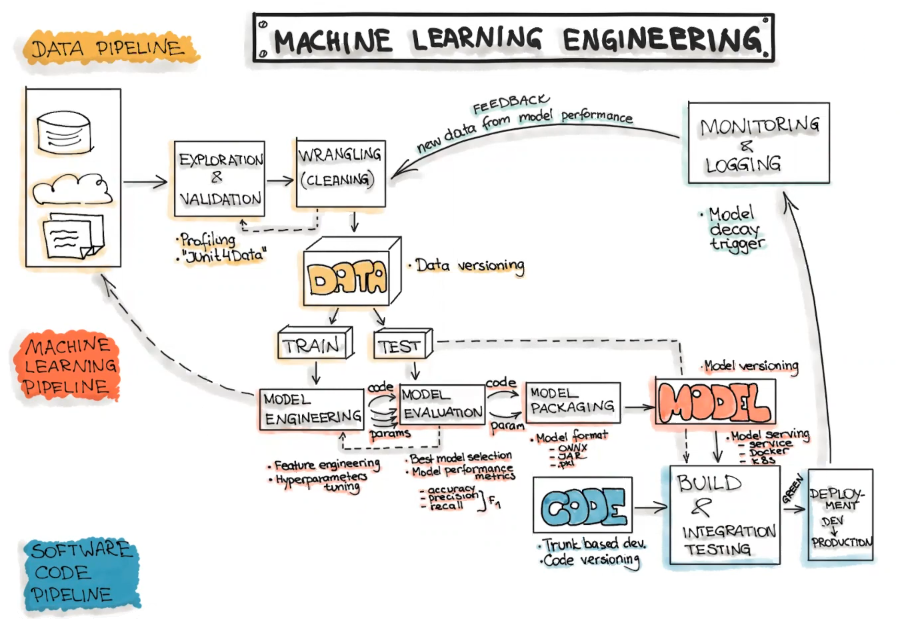
\includegraphics[scale=0.55]{architecture.png}
    \caption{Arquitectura MLOps}
    \label{fig:architecure-mlops}
\end{figure}

\subsection{Principios de MLOps}
A continuación, vamos a detallar los principios de MLOps que vamos a seguir en el desarrollo de nuestro proyecto.
En esta sección se incluyen los puntos más importantes de la metodología, durante todo el desarrollo intentaremos
cumplir con ellos en la medida de lo posible, ya que pueden darse situaciones en las que sea totalmente imposible
satisfacerlos al completo.

\begin{itemize}
    \item \textbf{Automatización}: la automatización es la clave para la eficiencia y la escalabilidad.
          Aqui incluimos tareas como la generación de datos, el despliegue del modelo, la evaluación y
          la puesta en producción.
    \item \textbf{Testeo}: garantiza que tanto la funcionalidad como el desempeño del modelo están evaluados correctamente.
          Esencial en Machine Learning para identificar problemas y mejorar la confianza en los resultados.
    \item \textbf{Versionado}: es importante tener un control de versiones de los datos, el código y los modelos.
          Puede variar el método dependiendo de la herramienta que se utilice, pero existen estándares como Git para la gestión
          de código y GitHub/GitLab para el almacenamiento de los repositorios.
    \item \textbf{Reproducibilidad}: es necesario poder reproducir los resultados de forma consistente, puede ser
          complicado en Machine Learning debido a la naturaleza aleatoria de los algoritmos. Igualmente aquí se trataran
          las herramientas y medidas necesarias para lograrlo.
    \item \textbf{Monitorización}: es importante tener un control de los modelos en proceso de entrenamiento o de producción.
          Por ello, recolectar estadisiticas en tiempo de procesamiento nos ayudará a generar nuevas hipotesis para las proximas interaciones.
\end{itemize}

\subsection{Metodología de trabajo}
Una de las características de los proyectos de Machine Learning es que son tecnologías en constante evolución, el
desarrollo no es un proceso sencillo y requiere de un enfoque coordinado por parte de los diferentes
equipos que lo conforman para asegurar su sostenibilidad a largo plazo. Es fundamental poder adapatarse a los cambios
de forma agil, sin que esto suponga un deterioro del nivel de productividad o que ralentice el avance de nuevas
funcionalidades.\medskip

Podemos identificar tres fases principales: diseño, desarrollo del modelo y operaciones. Cada fase tiene un enfoque
específico y requiere una serie de tareas para garantizar el éxito del proyecto. La fase de diseño,
se definen los objetivos y requisitos del proyecto, se identifican los datos necesarios para el entrenamiento y
se establecen los criterios de éxito. La fase de desarrollo del modelo, se preparan los datos, se entrena el modelo
y se evalúa su rendimiento. También se realiza la validación y se toman las decisiones sobre el modelo final a utilizar.
Finalmente, en la fase de operaciones, se integra el modelo en la infraestructura existente, se monitorea su rendimiento
y se extraen conclusiones para futuras iteraciones. Al repartir las responsabilidades en diferentes fases, aislamos los erroes junto con la carga de trabajo y podemos avanzar
sin la preocuapacion de que un bug o un cambio requisitos afecte al resto del equipo.

\begin{figure}[ht]
    \centering
    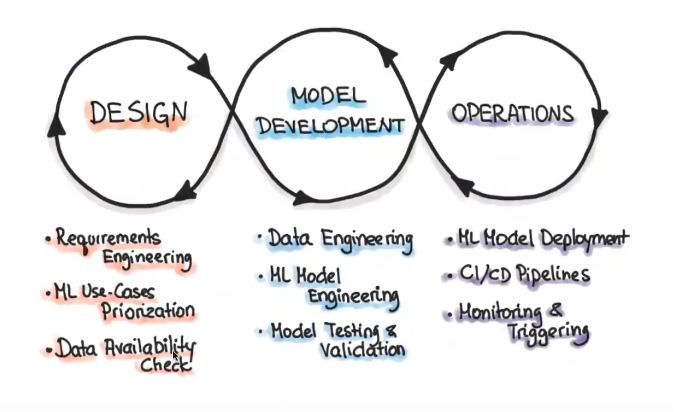
\includegraphics[scale=0.5]{proceso-mlops.png}
    \caption{Metodología MLOps}
    \label{fig:proces-mlops}
\end{figure}

Para visualizar de forma más clara la ventaja que supone este enfoque frente a uno tradicional, a continuación
se mencionara un ejemplos de una posible situacion real. \textbf{Ejemplo:} Tenemos un modelo que actualmente está alojado en AWS y queremos migrarlo a Azure, debido a que
utilizamos MLOps existe configurada una action que en el momento que el equipo publica una nueva release
automáticamente despliega el modelo en el servidor cloud. La parte del equipo encargada de las operaciones procede
a configurar el nuevo servicio y modificar la action para redirigir el despliegue al nuevo servidor. Durante este
tiempo, el equipo de desarrollo a podido avanzar en nuevas mejoras para el modelo y ahora se disponen a volver
a publicar los cambios. Ellos no han notado ningún cambio, pero a nivel de infraestructura se ha realizado una
completa migracion sin afectar en ningún momento en el desarrollo.


\pagebreak
    \section{Herramientas de desarrollo}
    La siguiente sección se enfoca en presentar las herramientas utilizadas para el desarrollo y  
    mantenimiento del codigo fuente del proyecto. Los recursos que se mencionan, si vien ayudan positivamente 
    al ecosistema de trabajo y a la calidad del mismo, es importante destacar que en este apartado no se incluyen 
    detalles sobre ninguna tecnologia directamente relacionada con la implementación del modelo de Machine Learning. 
    Este aspecto se tratará en un apartado posterior del informe.

    \subsection{Jupyter Notebook}

    \subsection{Pyenv y Virtualenv}

    \subsection{Git}

    \subsection{Pip-tools}

    \subsection{Pytest}
    Pytest es una de las mejores opciones para el testing de software y la preferente en proyectos de Python. 
    Es la libreria más popular dentro del Machine Learning debido a su facilidad de uso y  
    permite escribir teses unitarios de forma funcional. Cuenta con una amplia variedad 
    de herramientas para la gestion de pruebas, algunos de sus utilidades más relevantes son las fixtures, que
    optimiza la reutilización de recursos; el mock, que encapsula la funcionalidad de una funcion para poder
    testearla de forma aislada y el coverage, que muestra que zonas del codigo están cubiertas por la suit de teses. 

    \subsection{Pre-commit}

    \subsection{Makefile}

    \subsection{Flake8}

    \subsection{Black}
    
    \subsection{Docker}
    

\pagebreak
    \section{Sistema de evaluación del modelo}
    Un buen sistema de evaluación es esencial para un proyecto de machine learning. 
    No solo es útil por el hecho de medir la precisión y el rendimiento de los modelos, 
    sino que además sirve como un identificador claro de nuestro progeso dentro del desarrollo. 
    El seleccionar el modelo óptimo en fases tempranas del proceso no es tan importante 
    como el saber que las iteraciones en las que gastamos tiempo y recursos estan teniendo un impacto 
    positivo en su aprendizaje. Aunque físicamente es imposible conseguir una productividad 
    perfecta, con ayuda de una metodología sólida es posible reducir al maximo esta problemática.
    
    \subsection{Selección de métrica}
    El objetivo de una métrica es, mediante ponderacion numérica, identificar errores en el modelo y 
    servir como ayuda para la toma de decisiones, cambios en el diseñe o la soluación de problemas. En el caso del 
    FJSP, el objetivo es encontrar una acorde a la tarea que queramos abordar. En la literatura se atacan dos puntos
    principalmente: \textit{minimizar el tiempo de finalización} y \textit{minimizar el tiempo de espera entre máquinas}. 

    \begin{itemize}
        \item \textbf{Minimizar el tiempo de espera entre máquinas:} mide el tiempo promedio que cada operación debe 
        esperar antes de ser procesado en una máquina específica. Esta métrica es importante porque 
        indica la eficiencia del sistema en términos de cómo se están utilizando los recursos disponibles 
        y cómo se gestionan los trabajos en las colas.
        \item \textbf{Minimizar el tiempo de finalización:} se basa en el tiempo total que se tarda en completar todos 
        los trabajos del sistema. Es un buen indicador porque evalúa el rendimiento global del sistema 
        y la eficacia para completar el proceso en el plazo establecido. 
    \end{itemize}

    Aunque ambas métricas son importantes, la segunda es la que se vamos a utilizar como referencia en cuanto al
    desempeño del modelo, ya que uno de nuestros objetivos principales es reducir los tiempos de producción y no tanto
    aprobechar las máquinas lo máximo posible. Es posible utilizar ambas para identificar puntos débiles tanto del modelo 
    como del propio proceso que se quiere optimizar pero, por la propia idiosincrasia de las mismas, el mejorar la puntuación
    en una de ellas inevitablemente afectara negativamente la puntuación de la otra en un amplio número de casuísticas.

    \subsection{Implementación de la métrica} 


\pagebreak
    \section{Modelado del problema}
El modelado del problema es una de los campos con mayor potencial dentro del FJSP, el tener una propuesta
solida con la que trabajar repercutirá directamente en los resultados finales, por lo que es necesario
contemplar diferentes propuestas y hacer una valoración objetiva.

\subsection{Reinforcement Learning}
Nuestra solucion se basa en la decisión de utilizar Reinforcement Learning (RL), ya que puede ser útil a la hora
de resolver este tipo de problemas de optimización combinatoria. El RL es un tipo de aprendizaje automático que
se basa en la interacción de un agente con un entorno. El agente toma decisiones en función de la información
que recibe del entorno y obtiene una recompensa o penalización acorde a las decisiones que toma. El objetivo
del agente es maximizar la recompensa total obtenida a lo largo del tiempo. Este tipo de técnicas se pueden
utilizar para resolver problemas de optimización combinatoria en los que el espacio de estados es muy grande
y no es posible explorar todas sus combinaciones. En este tipo de problemas, el RL puede ser útil para encontrar
soluciones óptimas (o aproximaciones) sin necesidad de explorar todo el espacio de estados.

Nuestro agente puede ser entrenado para tomar decisiones óptimas, estas acciones haran referencia a la
asignación de tareas a máquinas y su objetivo será aprender a proveer de una solución al problema.
Es especialmente interasante el uso de RL ya que solución del problema a cambios en el entorno, como cambios en la disponibilidad
de máquinas o en la duración de las tareas. El agente puede aprender a reaccionar de manera óptima a estos
cambios en tiempo real. En casos en los que el espacio de estado del problema es muy grande o cambia continuamente,
el aprendizaje por refuerzo puede ser útil para encontrar soluciones óptimas sin necesidad de
explorar todo el espacio de estado. Esto puede ser especialmente útil en problemas de programación de taller de trabajo
flexible con un gran número de máquinas y tareas. Dentro de un entorno de reinforcement learning, es necesario definir
una serie de elementos: el agente, encargado de interactuar con el entorno; el estado, representación del problema;
las acciones, interacción del agente con el entorno y el reward, recompensa asociada a las decisiones del agente.


\subsection{Estado del environment}
La justificación de usar PyTorch Geometrics es que ofrece soporte para el procesamiento de grafos,
lo que significa que se puede utilizar para trabajar con redes de datos en las que los nodos están
conectados por enlaces. Esto puede ser útil porque mediante técnicas de Deep Learning se puede analizar
la estructura y las relaciones que existen entre los nodos de un grafo. Además, la librería ofrece herramientas
para trabajar con diferentes tipos de grafos, como grafos dirigidos y heterogéneos, que son los utilizados en
nuestra representación, y proporciona una serie de funciones para realizar operaciones básicas con grafos.

    \printbibliography[title=Bibliografía]

\end{document}